\documentclass[a4paper,11pt]{article}
\usepackage{color}
\usepackage{graphicx}
\usepackage{subcaption}
\usepackage{amsmath}
\usepackage{tikz}
\usepackage{listings}
\definecolor{codegreen}{rgb}{0,0.6,0}
\definecolor{codegray}{rgb}{0.5,0.5,0.5}
\definecolor{codepurple}{rgb}{0.58,0,0.82}
\definecolor{backcolour}{rgb}{0.95,0.95,0.92}
 
\lstdefinestyle{mystyle}{
    backgroundcolor=\color{backcolour},   
    commentstyle=\color{codegreen},
    keywordstyle=\color{magenta},
    numberstyle=\tiny\color{codegray},
    stringstyle=\color{codepurple},
    basicstyle=\footnotesize,
    breakatwhitespace=false,         
    breaklines=true,                 
    captionpos=b,                    
    keepspaces=true,                 
    numbers=left,                    
    numbersep=5pt,                  
    showspaces=false,                
    showstringspaces=false,
    showtabs=false,                  
    tabsize=2
}
 
\lstset{style=mystyle}
\usetikzlibrary{automata,positioning}

\graphicspath{ {images/} }
\begin{document}
\title{\color{red}CARNEGIE MELLON UNIVERSITY\\
APPLIED STOCHASTIC PROCESSES  (COURSE 18-751)\\
HOMEWORK 5}
\author{Daniel Marew}
\date{\today}
\clearpage\maketitle

\thispagestyle{empty}
\newpage
I collaborated with :\\
\hspace*{6cm}
Nebyou Yismaw\\
\hspace*{6cm}
Daniel    Nkemelu\\
\hspace*{6cm}
Agatha Niwomugizi
\thispagestyle{empty}
\newpage
\clearpage
\setcounter{page}{1}
\section*{Q.1}
\subsection*{(a)}
The codeword is in error when there are more than $e$ errors\\
$\implies$
$$P_{codeerror} =\sum_{j=e+1}^{n} \binom{n}{j}p^j(1-p)^{n-j}$$
\subsection*{(b)}
The most significant term in $P_{codeerror}$ is the first one.i.e when $j = e+1$\\\\
$\implies$\\\\
$$P_{codeerror} \approx \binom{n}{e+1}p^{e+1}(1-p)^{n-e-1}$$
For small $p$ and $N<100$\quad $1-p \approx 1$ \\\\
$\implies$\\
$$P_{codeerror} \approx \binom{n}{e+1}p^{e+1}$$
\subsection*{(c) Bit Error Rate}
$$P(biterror|codeerror) \approx \frac{1}{2}$$
$$\implies  P(biterror) = P(biterror|codeerror)P_{codeerror}+P(biterror|Nocodeerror)P(Nocodeerror)$$
Since $P(biterror|Nocodeerror) = 0$
$$ P_{biterror} = P(biterror|codeerror)P_{codeerror}$$
$$ P_{biterror} \approx \frac{1}{2}P_{codeerror}$$
$$ P_{biterror} \approx \frac{1}{2}\sum_{j=e+1}^{n} \binom{n}{j}p^j(1-p)^{n-j}$$
\newpage
\clearpage
\subsection*{(d)}
\textbf{BER for [1,1,0]}\\\\
It is the same as sending a single bit across the channel hence, BER is the same as the channel bit rate\\
$\implies P_{biterror}=p$\\
$ p = 0.01 \implies P_{biterror} = 0.01$\\
$ p = 0.001 \implies P_{biterror} = 0.001$\\
$ p = 10^{-6} \implies P_{biterror} = 10^{-6}$\\\\
\textbf{BER for [7,4,1]}\\\\
$$P_{biterror}  = \frac{1}{2}P_{codeerror}$$
$$ P_{biterror} = \frac{1}{2}\sum_{j=1+1}^{7} \binom{7}{j}p^j(1-p)^{7-j}$$
$$ = \frac{1}{2}(1-\sum_{j=0}^{1} \binom{7}{j}p^j(1-p)^{7-j})$$
$$ = \frac{1}{2}(1- \binom{7}{0}(1-p)^7 - \binom{7}{1}(1-p)^6)$$
$$ = \frac{1}{2}(1- (1-p)^7 - 7(1-p)^6)$$
$p = 0.01 \implies$ $P_{biterror} = \frac{1}{2}(1- (1-0.01)^7 - 7(1-0.01)^6) = 0.001$\\
$p = 0.001 \implies$ $P_{biterror} = \frac{1}{2}(1- (1-0.001)^7 - 7(1-0.001)^6) = 1.04x10^{-5}$\\
$p = 10^{-6} \implies$ $P_{biterror} = \frac{1}{2}(1- (1- 10^{-6})^7 - 7(1- 10^{-6})^6) =  1.05x10^{-11}$
\subsection*{(e)}
[1,1,0] has the same bit error rate as the channel\\
$\implies p = 10^{-6}$  \\\\
For [7,4,1]\\
$$P_{biterror} = \frac{1}{2}P_{codeerror}$$
$$P_{biterror} = \frac{1}{2}\binom{n}{e+1}p^{e+1} = 10^{-6}$$
$$\implies p^{e+1} = \frac{2x10^{-6}}{\binom{n}{e+1}}$$
$$ p^{2} = \frac{2x10^{-6}}{\binom{7}{2}}$$
$$p = \sqrt{\frac{2x10^{-6}}{\binom{7}{2}}}$$
$$p = 3.08x10^{-4}$$
\newpage
\clearpage
\section*{Q.2}
\subsection*{(a) Compute the MAP and MLE decision boundaries}
we can get the MAP decision boundary by finding such that 
\begin{equation}
\frac{f_{r|0}p(0)}{f_{r|1}p(1)}>1
\end{equation}• 
\begin{equation}
f_{r|0} = \frac{1}{\sqrt{2\pi}}e^\frac{-(x+a)^2}{2}
\end{equation}•
\begin{equation}
f_{r|1} = \frac{1}{\sqrt{2\pi}}e^\frac{-(x-a)^2}{2}
\end{equation}•
$\implies$
$$\frac{e^\frac{-(r-a)^2}{2}(1-p)}{e^\frac{-(r+a)^2}{2}p}>1$$
$$e^\frac{-(r-a)^2+(r+a)^2}{2}>\frac{p}{1-p}$$
$$e^{-2ar}>\frac{p}{1-p}$$
$$-2ar>ln\frac{p}{1-p}$$
$$r<\frac{-1}{2a}ln\frac{p}{1-p}$$
$$r<\frac{1}{2a}ln\frac{1-p}{p}$$
That means when $r<\frac{1}{2a}ln\frac{1-p}{p}$ we interpret it as 0 else we interpret it  as a 1.\\
$MLE = MAP$ when $p = 1-p$\\
$\implies$
$$r<\frac{1}{2a}ln\frac{p}{p}\implies r<0$$
So the MLE decision boundary is $r=0$
\clearpage
\newpage
\subsection*{(b)}
\begin{figure}[h]
   \hspace*{-5.5cm}
    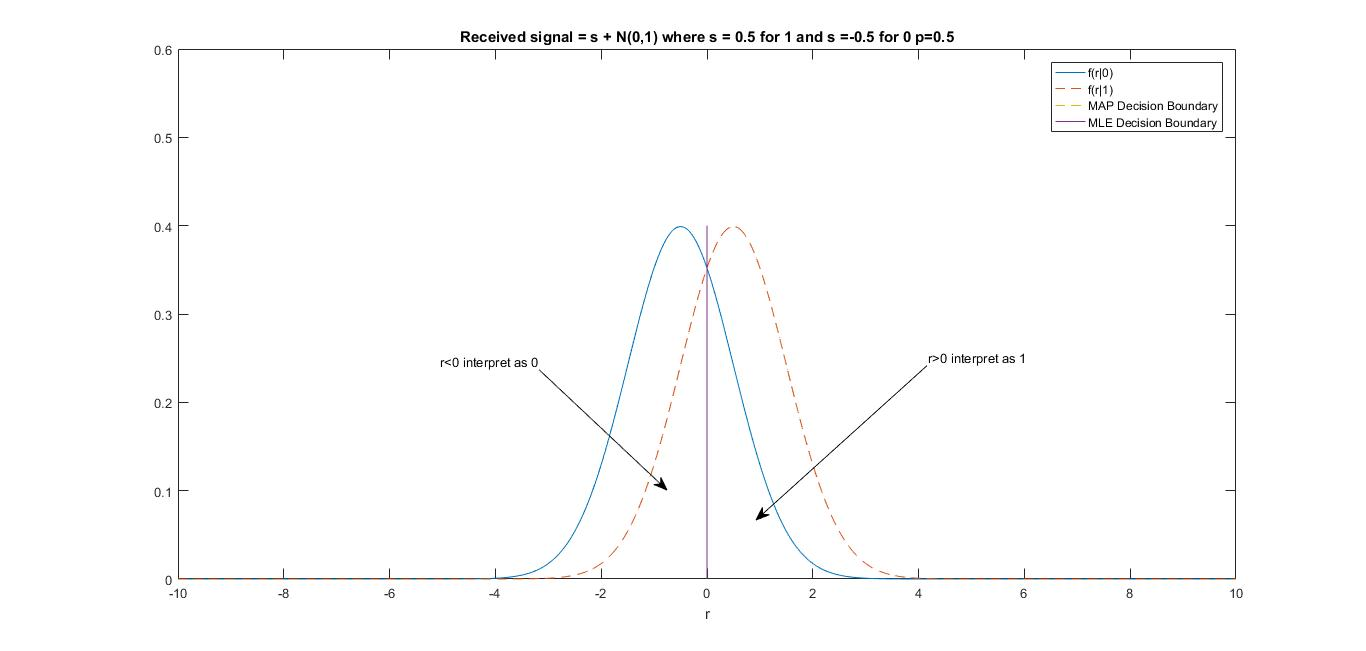
\includegraphics[scale=0.5]{q2_b_1}
    \caption{pdf of r , MAP and MLE decision boundaries when $p=0.5$ and $a=0.5$}\label{fig:q2_b_1}
\end{figure}
\begin{figure}[h]
   \hspace*{-5.5cm}
    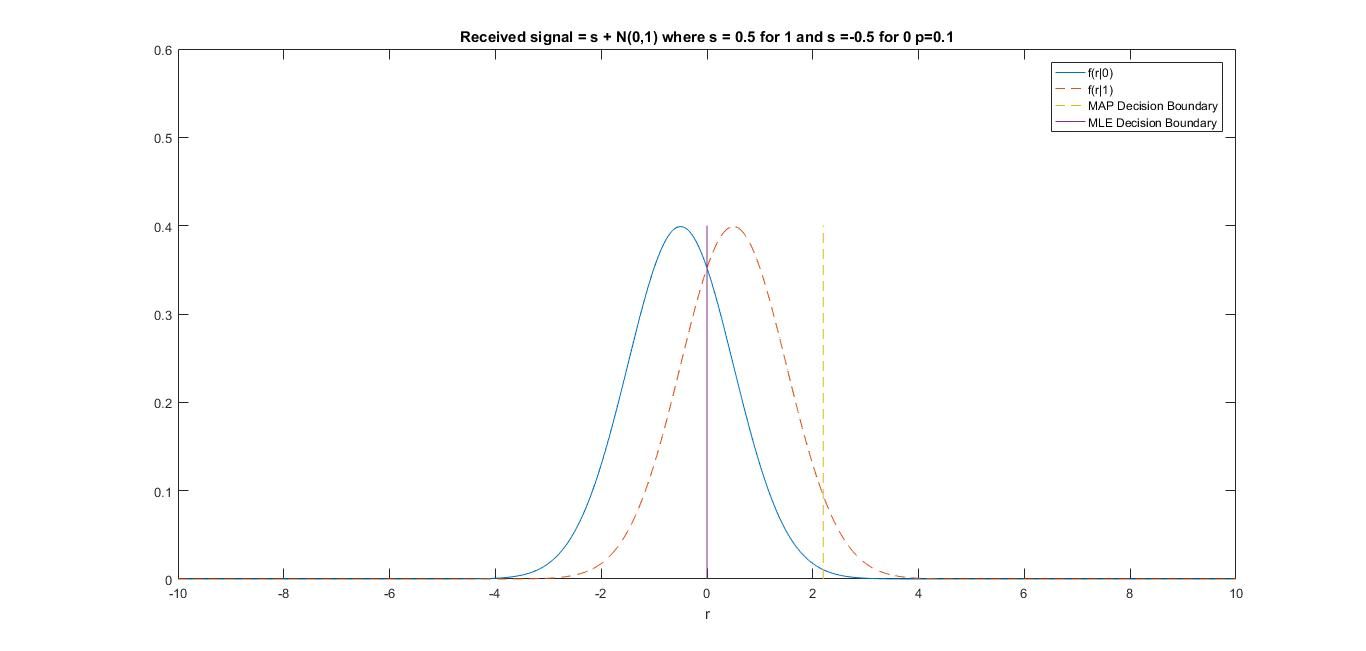
\includegraphics[scale=0.5]{q2_b_2}
    \caption{pdf of r , MAP and MLE decision boundaries when $p=0.1$ and $a=0.5$}\label{fig:q2_b_2}
\end{figure}
\clearpage
\newpage
\subsection*{(c) Compute the expected bit error rate}
$$P(biterror) = P(biterror|1)P(1)+P(biterror|0)P(0)$$
$$P(biterror|0) = \int_{\beta}^{\infty}f_{r|0}(r) dr$$
$$P(biterror|1) = \int_{-\infty}^{\beta}f_{r|1}(r) dr$$
where $\beta$ is the decision boundary.\\
If we have a normal variable $X\sim N(\mu,\sigma^2)$, the probability that $X>x$ is\\
\begin{equation}
Pr\{X>c\} = Q(\frac{x-\mu}{\sigma})
\end{equation}•
where Q is the Q-function\\
$\implies$

$$P(biterror|0) = \int_{\beta}^{\infty}f_{r|0}(r) dr = Q\bigg(\frac{\beta-(-a)}{1}\bigg)= Q\big(\beta+a\big)$$
similarly,
$$P(biterror|1) = \int_{-\infty}^{\beta}f_{r|1}(r) dr=1-\int_{\beta}^{\infty}f_{r|1}(r) dr=1-Q\bigg(\frac{\beta-a}{1}\bigg)=1-Q\big(\beta-a\big)$$
$$P(biterror) = P(0)Q\big(\beta+a\big)+P(1)(1-Q\big(\beta-a\big))$$\\\\
 MAP decision boundary and $p=0.5$ $\implies \beta = 0$  \\\\
 $$P(biterror) = P(0)Q\big(0+a\big)+P(1)(1-Q\big(0-a\big)) =0.5(Q(a)+(1-Q(-a)))  $$
 $$Q(-a) = 1 - Q(a)$$
 $$P(biterror) =0.5(Q\big(a\big)+(1-(1-Q(a)))) =Q(a) $$
 for a = 0.5 bit error rate  $= P(biterror) =Q(a) = Q(0.5) = 0.3085$\\\\
 MLE decision boundary  $\implies \beta = 0$  the same as MAP above for a = 0.5 bit error rate  $= P(biterror) =Q(a) = Q(0.5) = 0.3085$\\\\
 MAP decision boundary a=0.5 and $p=0.1$\\ $\implies$\\
 $$\beta =\frac{1}{2a} ln\frac{1-p}{p}=ln\frac{0.9}{0.1}=2.1972$$
 $$P(biterror) = 0.9Q\big(2.1972+a\big)+0.1(1-Q\big(2.1972-a\big))
 $$
 $$= 0.9Q\big(2.1972+0.5\big)+0.1(1-Q\big(2.1972-0.5\big)) $$
 $$= 0.9Q\big(2.6972\big)+0.1(1-Q\big(1.6972\big)) $$
 $$= 0.9*0.0035+0.1(1-0.0448)=0.0987 $$
 for $a = 0.5$ and $p=0.1$  bit error rate  $= P(biterror) = 0.0987$  MAP decision boundary\\\\
 MLE decision boundary $\implies \beta =0$ \\
 $$P(biterror) = 0.9Q\big(a\big)+0.1(1-Q\big(-a\big))$$
 $$P(biterror) = 0.9Q(a)+0.1(1-(1-Q(a)))$$
 $$=0.9Q(0.5)+0.1(1-(1-Q(0.5))) = 0.3085$$
 for $a = 0.5$ and $p=0.1$  bit error rate  $= P(biterror) =  0.3085$ with MLE decision boundary\\\\
 \subsection*{(d) ROC}
 \begin{figure}[h]
   \hspace*{-1cm}
    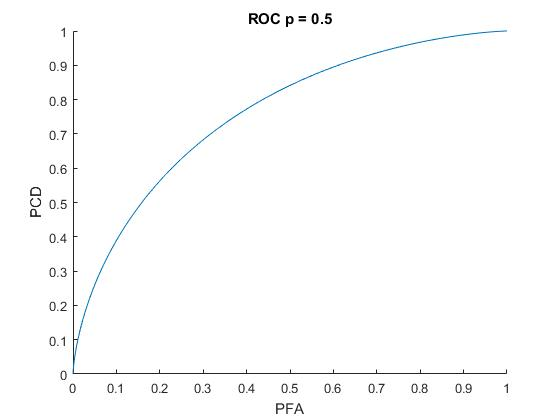
\includegraphics[scale=0.5]{q2_d_2}
    \caption{ROC for $a=0.5$,$p=0.5$}\label{fig:q2_d_1}
\end{figure}
 \begin{figure}[h]
   \hspace*{-1cm}
    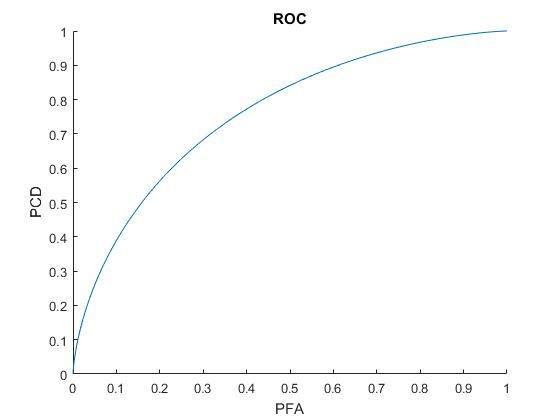
\includegraphics[scale=0.5]{q2_d_1}
    \caption{ROC for $a=0.5$ $p = 0.1$}\label{fig:q2_d_1}
\end{figure}
\clearpage
\newpage
\section*{Q.3}
\subsection*{(a) Code [1,1,0]}
With MAP decision boundary when $p = 0.5$ \\
bit error rate  $= P(biterror)=P(codeerror) =Q(a)$ from 2.c\\\\
$\implies$\\
$$Q(a) = 10^{-6}$$
$$a = Q^{-1}(10^{-6})$$
$$a =4.7534$$
Average energy per bit $= \beta a^2=22.5950\beta$
\subsection*{(b) Code [7,4,1]}
With MAP decision boundary when $p = 0.5$ \\
$P(codeerror) =Q(a)$ from 2.c and $P(biterror) = \frac{1}{2}P(codeerror)$ from 1.c \\\\
$$P(codeerror) = 2P(biterror) = 2*10^{-6}$$
$\implies$\\
$$Q(a) = 2*10^{-6}$$
$$a = Q^{-1}(2*10^{-6})$$
$$a =4.6114$$
For every 4 bit we send 7 bit long codeword. That means for every bit we will need
$\frac{7}{•4}$x(the energy to send a single bit) energy.\\\\
Average energy per bit $= \frac{7}{4}\beta a^2=37.2135\beta$
\subsection*{(c) Which of the two codes is the most efficient and by what factor}
From energy consumption perspective (a) is more efficient.\\
$factor =$ Average energy per bit (b)/ Average energy per bit (a) $=\frac{37.2135\beta}{22.5950\beta}$\\
$factor =1.6469$\\
i.e with the second code [7,4,1] we will need 1.6469 times more energy than [1,1,0]. 









\end{document}